\section{CHƯƠNG 8: DASHBOARD PHÂN TÍCH XU HƯỚNG}

\subsection{Giới thiệu và Tổng quan dữ liệu}

Dashboard này được thiết kế nhằm cung cấp công cụ khám phá và theo dõi xu hướng đề cập của các món ăn và địa điểm ẩm thực dựa trên dữ liệu video TikTok. Bộ dữ liệu ban đầu được thu thập từ các video của các TikToker chuyên về ẩm thực, với tổng số \textbf{hơn 70,000} video. Quá trình thu thập diễn ra liên tục trong vòng \textbf{70 tuần}, từ \textbf{Tuần 47 Năm 2023} (tháng 11/2023) đến \textbf{Tuần 12 Năm 2025} (tháng 03/2025). Để thu gọn quy mô và đảm bảo bộ dữ liệu phản ánh các xu hướng nổi bật của từng tuần, nhóm đã tiến hành chọn lọc: mỗi tuần chỉ giữ lại \textbf{20\%} video có \textbf{điểm số cao nhất} (tiêu chí điểm số được trình bày chi tiết tại Mục~\ref{subsubsec:top_20_percent_video}). Nhờ quá trình chọn lọc này, bộ dữ liệu cuối cùng phần nào đại diện cho các món ăn và địa điểm \textbf{đã và đang phổ biến, thịnh hành} trên nền tảng trong suốt giai đoạn nghiên cứu.

\begin{figure}[H]
    \centering
    \frame{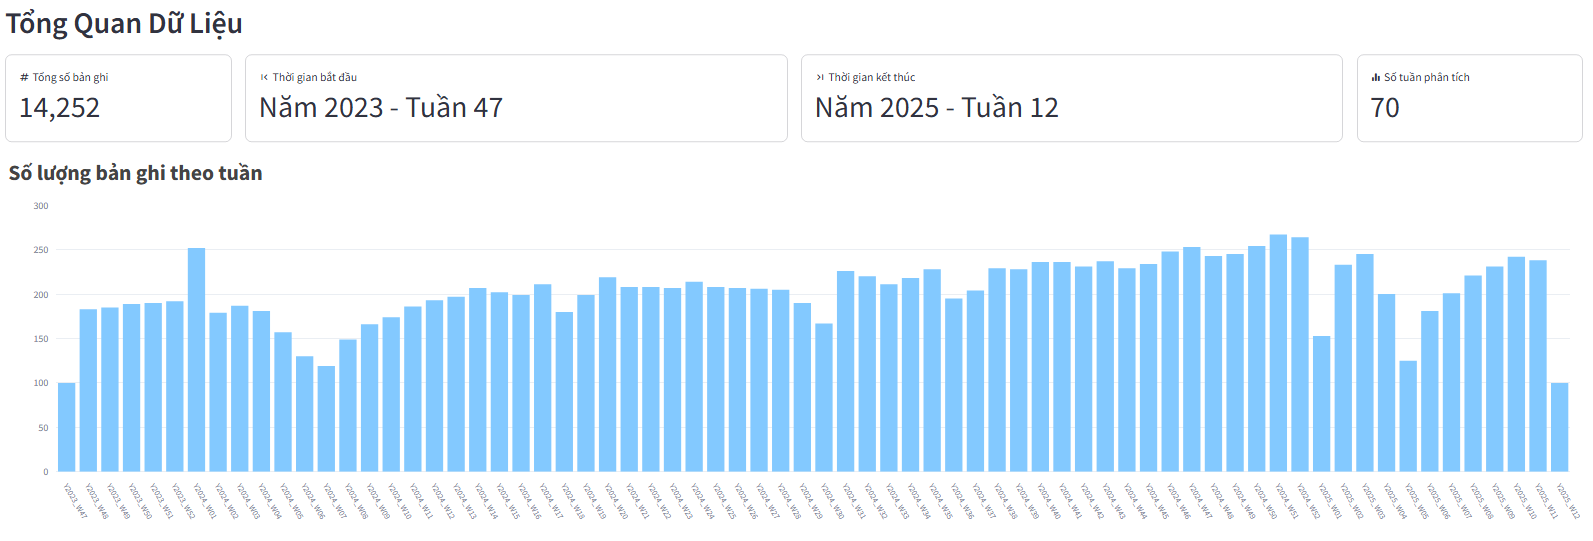
\includegraphics[width=0.95\textwidth]{img/tong_quan_du_lieu.png}}
    \caption{Tổng quan dữ liệu}
    \label{fig:tong_quan_du_lieu}
\end{figure}

\subsection{Phân tích Xu hướng theo thời gian}

\begin{figure}[H]
    \centering
    \frame{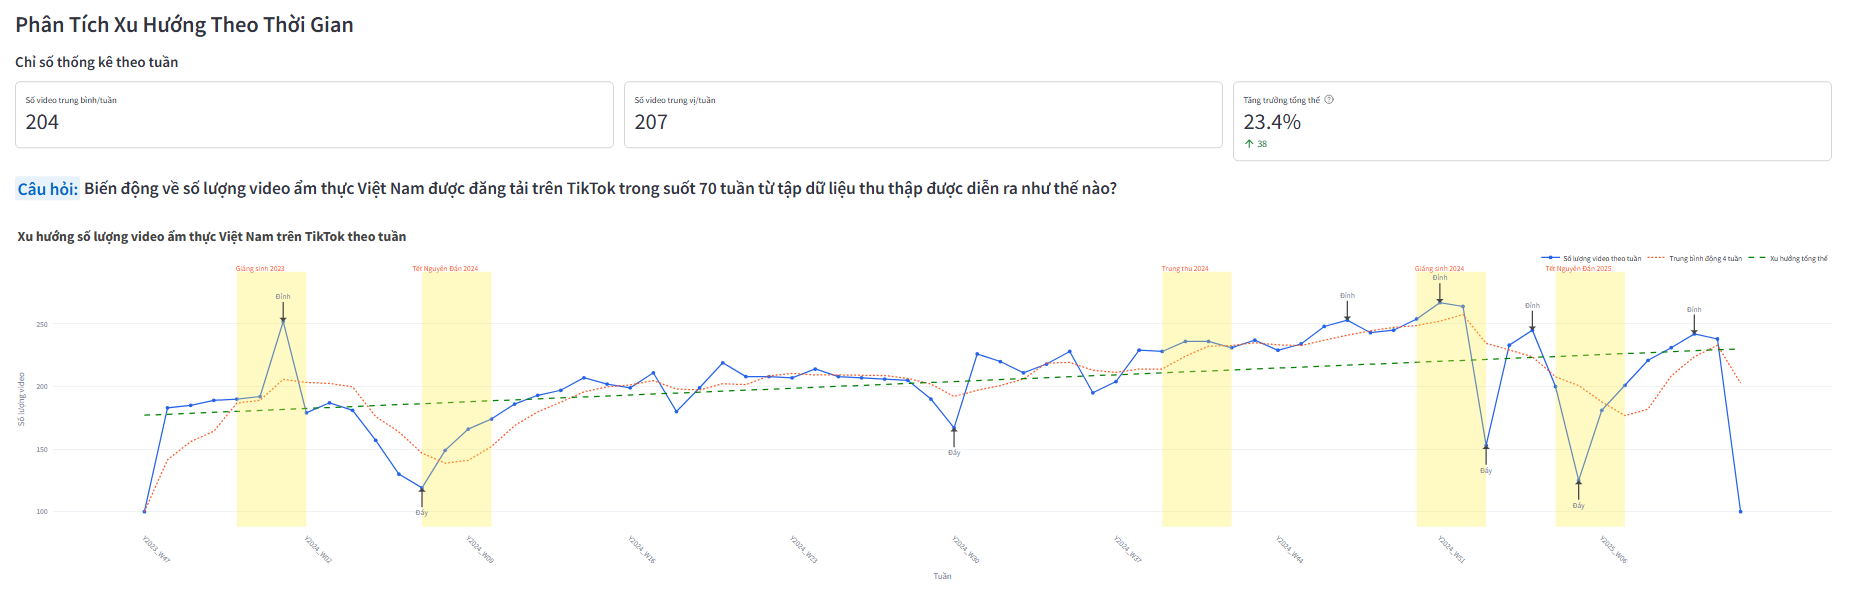
\includegraphics[width=0.95\textwidth]{img/xu_huong_thoi_gian.png}}
    \caption{Xu hướng theo Thời gian}
    \label{fig:xu_huong_thoi_gian}
\end{figure}

\paragraph{Nhận xét:}
\begin{enumerate}
    \item \textbf{Chỉ số thống kê theo Tuần:}
    \begin{itemize}
        \item Chỉ số thống kê theo tuần cho thấy số lượng video trung bình mỗi tuần đạt \textbf{204 video/tuần}, trung vị đạt \textbf{207 video/tuần}, thể hiện bộ dữ liệu không bị lệch quá nhiều và có thể kiểm tra lại với các phương pháp thống kê.
        
        \item Số lượng video cũng đạt mức tăng trưởng khoảng \textbf{23,4\%} khi so sánh 4 tuần đầu và 4 tuần cuối, phản ánh xu hướng quan tâm đến các video ẩm thực được gia tăng.
    \end{itemize}

    \item \textbf{Số lượng video qua từng giai đoạn:} Xem xét về sự biến động số lượng video theo từng giai đoạn, ta có thể thấy được số lượng video về ẩm thực xuất hiện nhiều nhất ở các Tuần Giáng Sinh và có xu hướng giảm dần cho đến thời điểm Tết Nguyên Đán vào năm sau.
\end{enumerate}

\subsection{Phân tích Phân bố địa lý}

\subsubsection{Phân bố Tỉnh/Thành phố được đề cập}

\paragraph{Tổng quan:}
Thông qua khảo sát dựa trên \textbf{14,252} bản ghi từ tập dữ liệu (xem Hình~\ref{fig:tinh_thanhpho}), chỉ khoảng \textbf{4,000} video có \textbf{đề cập đến địa điểm}. Trong đó, thành phố \textbf{Hà Nội} và thành phố \textbf{Hồ Chí Minh} là 2 thành phố được đề cập nhiều nhất trong toàn bộ dữ liệu ghi nhận được.

\begin{figure}[H]
    \centering
    \frame{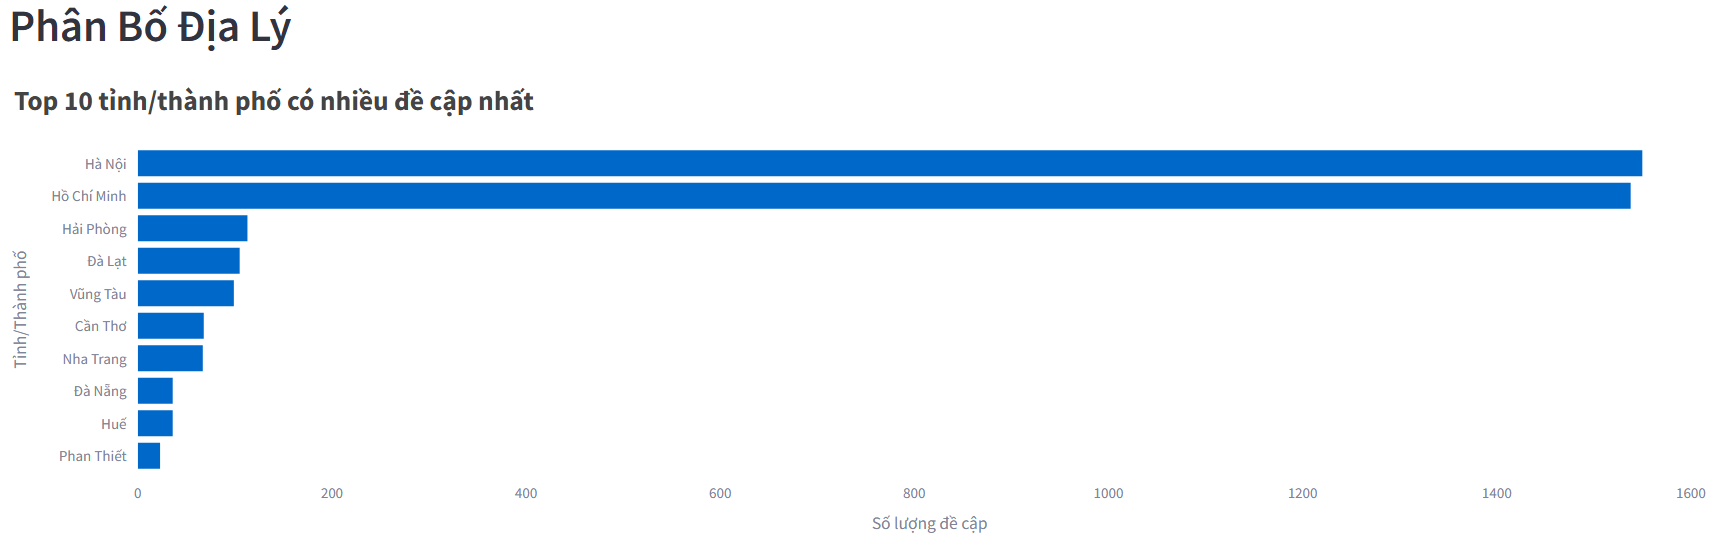
\includegraphics[width=0.99\textwidth]{img/tinh_thanhpho.png}}
    \caption{Phân bố các Tỉnh/Thành phố được đề cập}
    \label{fig:tinh_thanhpho}
\end{figure}

\paragraph{Phân tích chi tiết hơn:}
Hình~\ref{fig:muc_do_tap_trung} cho thấy: Số lượng video đề cập đến nhóm TP.Hồ Chí Minh và Hà Nội là \textbf{3088} (chiếm \textbf{78,94\%}), cao hơn đáng kể, gấp \textbf{3,75 lần} so với \textbf{824} đề cập (chiếm \textbf{21,06\%}) đến các địa phương khác. Kết quả kiểm định thống kê Mann-Whitney với $p=0.009 < 0.05$ đã xác nhận sự khác biệt này là có ý nghĩa thống kê, cho thấy mức độ tập trung đề cập vào hai thành phố lớn này là vượt trội so với tổng các tỉnh/thành phố còn lại.

\begin{figure}[H]
    \centering
    \frame{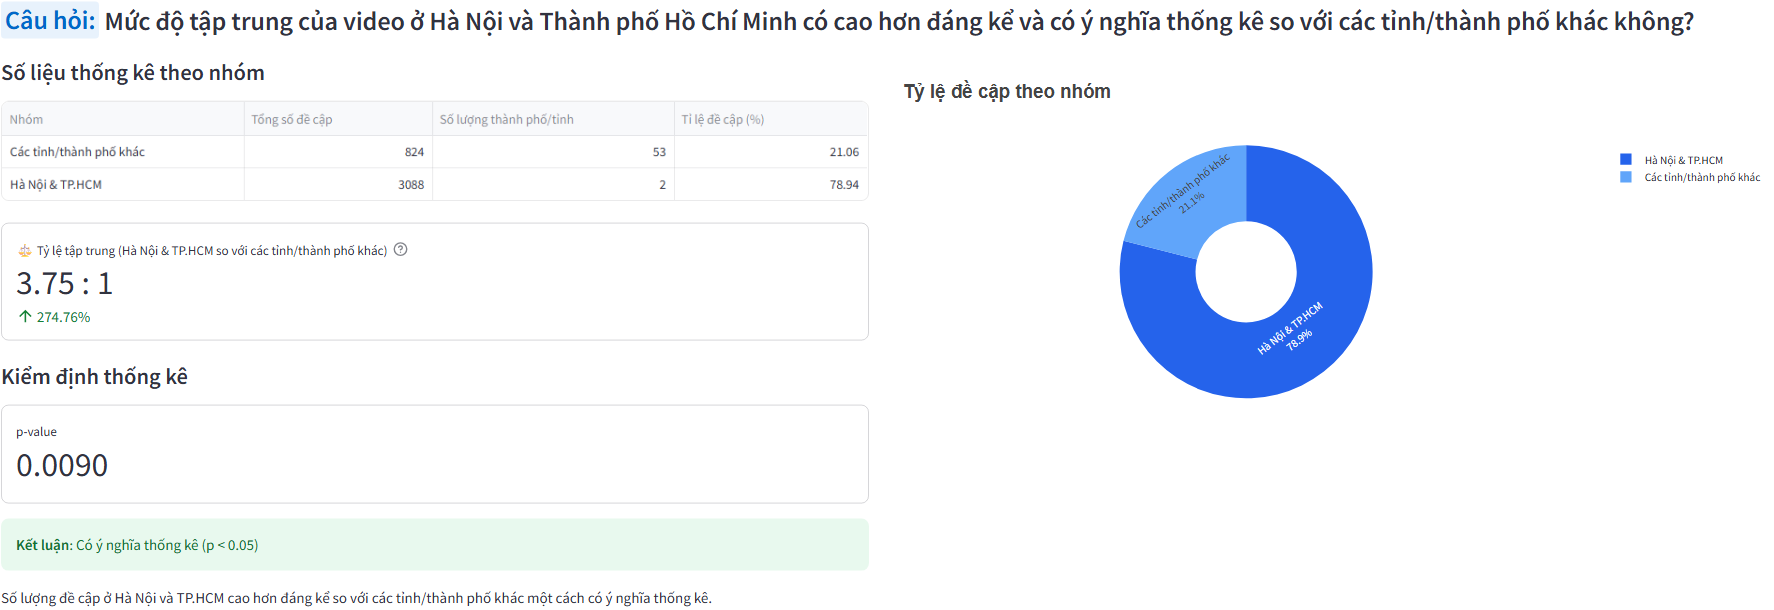
\includegraphics[width=0.99\textwidth]{img/muc_do_tap_trung.png}}
    \caption{Số lượng video đề cập đến TP.Hồ Chí Minh và Hà Nội so với các địa phương khác}
    \label{fig:muc_do_tap_trung}
\end{figure}

\subsubsection{Phân bố Tỉnh/Thành phố thuộc từng vùng miền}

\begin{figure}[H]
    \centering
    \frame{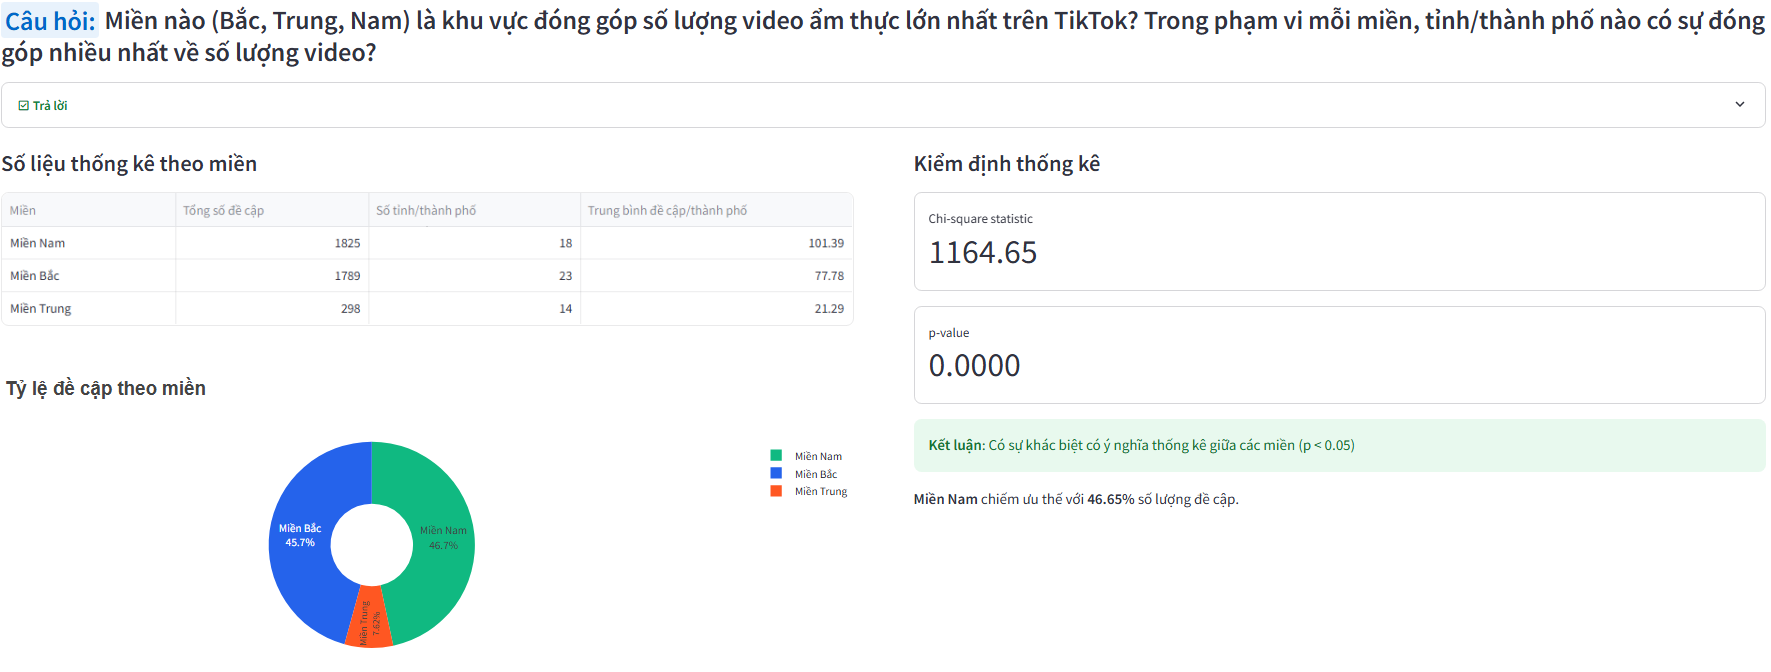
\includegraphics[width=0.99\textwidth]{img/video_mien.png}}
    \caption{Phân bố số lượng video theo từng miền}
    \label{fig:video_mien}
\end{figure}
\begin{figure}[H]
    \centering
    \frame{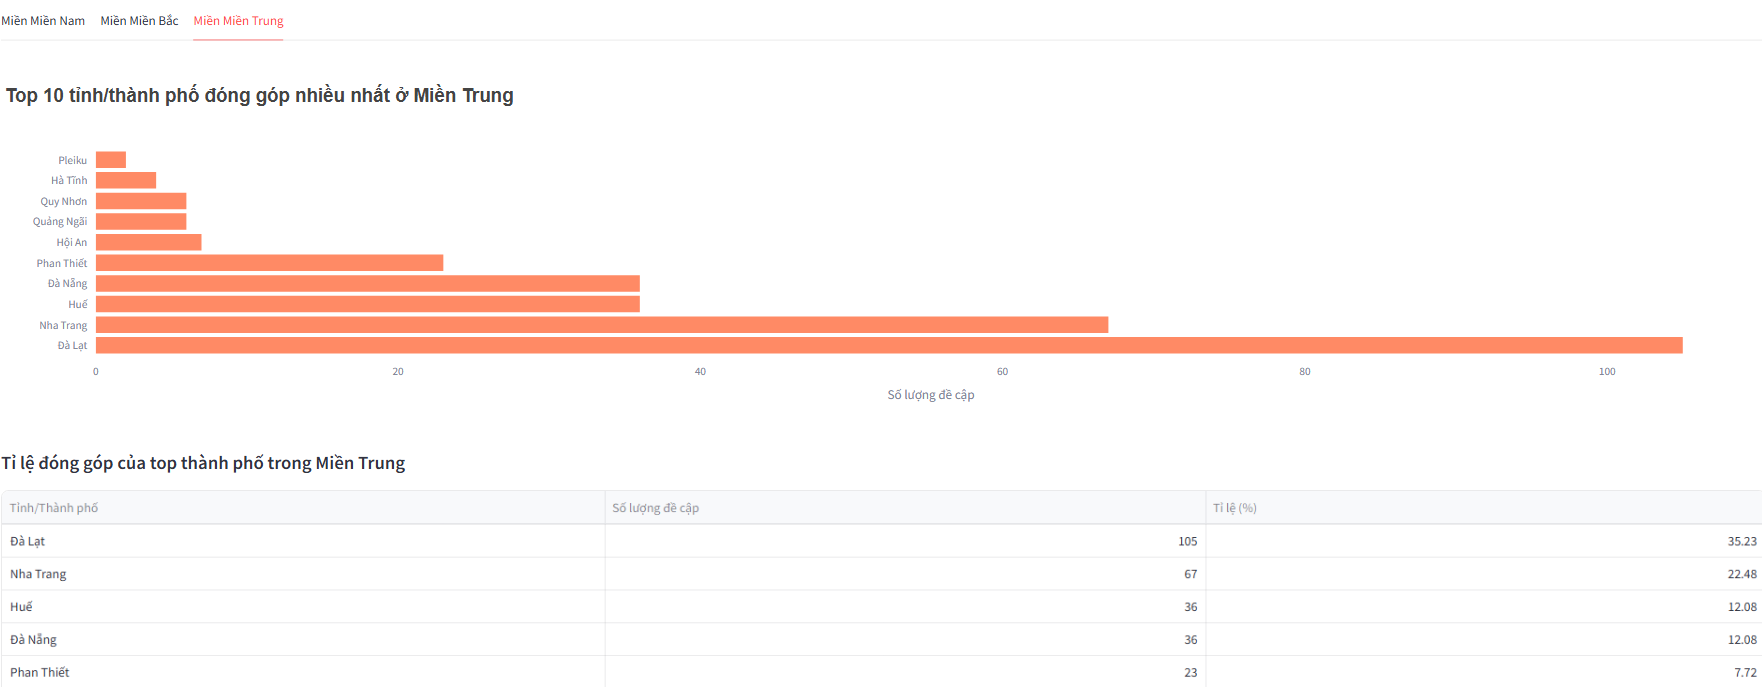
\includegraphics[width=0.99\textwidth]{img/thanhpho_mien.png}}
    \caption{Phân bố tỉnh/thành phố trong từng miền}
    \label{fig:thanhpho_mien}
\end{figure}

\paragraph{Nhận xét:} Sau khi chuẩn hóa địa điểm theo từng vùng miền (sử dụng quá trình \texttt{mapping}), ta nhận thấy sự phân bố số lượng video có sự khác biệt rõ rệt. Cụ thể, Miền Trung có số lượng video ít nhất (xem Hình~\ref{fig:video_mien}), chủ yếu tập trung vào các thành phố du lịch trọng điểm như Nha Trang, Đà Lạt, Huế (xem Hình~\ref{fig:thanhpho_mien}).

\paragraph{Kiểm định thống kê:} Để xác nhận liệu sự khác biệt trong phân bố số lượt đề cập giữa các vùng miền này có ý nghĩa thống kê hay không, nhóm đã tiến hành \textbf{kiểm định thống kê Chi-Square (Chi bình phương)}. Kết quả kiểm định đạt $\chi^2 = 1164.65$ và $p = 0.009 < 0.05$ (xem Hình~\ref{fig:video_mien}). Điều này \textbf{khẳng định rằng sự khác biệt về tỷ lệ/phân bổ số lượt đề cập giữa các danh mục (các vùng miền) là có ý nghĩa thống kê và không phải do ngẫu nhiên}. Dựa trên sự phân bố không đồng đều có ý nghĩa thống kê này, người dùng có thể xem xét phân tích và khai thác thị trường tiềm năng tại từng vùng miền.


\subsubsection{Phân bố Quận/Huyện thuộc Tỉnh/Thành phố}
\begin{figure}[H]
    \centering
    \frame{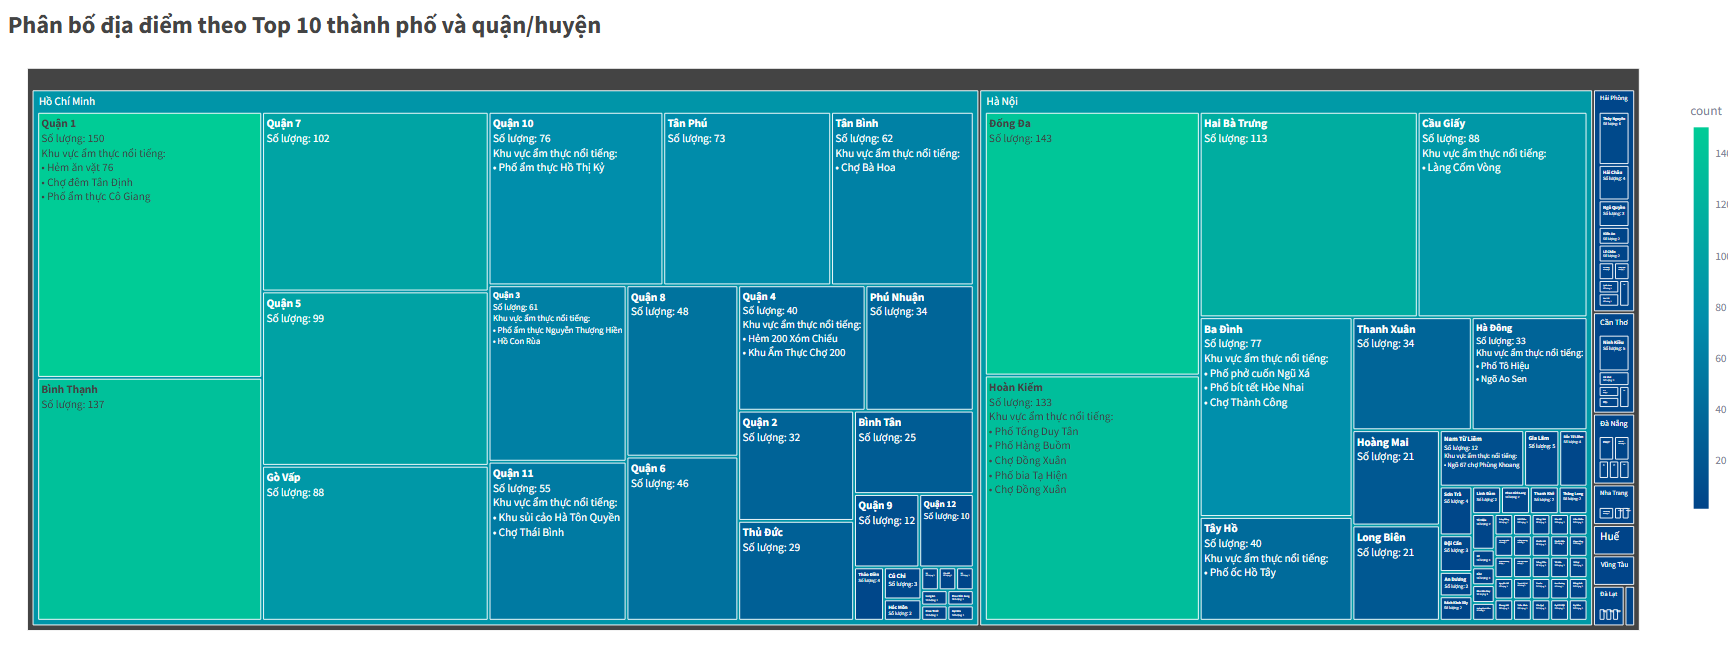
\includegraphics[width=0.99\textwidth]{img/quan_huyen.png}}
    \caption{Phân bố các Quận/Huyện thuộc Tỉnh/Thành phố}
    \label{fig:quan_huyen}
\end{figure}

Địa điểm được khảo sát từ tập dữ liệu sẽ là các \textbf{địa điểm được đề cập} chứ không đảm bảo đây là địa điểm chính xác trong video. Ví dụ, khi xử lý video có đoạn \textbf{transcript} bao gồm thông tin ``\textbf{Quán Bún đậu Hà Nội ở Quận 7}'', tập dữ liệu ghi nhận video chứa thông tin món ăn là Bún đậu, địa điểm thành phố Hà Nội và ở quận 7. 

Thông qua phân tích và đánh giá thủ công từ các video, nhóm sẽ xử lý phân loại địa điểm \textbf{dựa trên Quận/Huyện để đưa về Tỉnh/Thành phố} do nội dung mọi người đề cập thường là các quán ăn ở các địa điểm thuộc Quận/Huyện và có \textbf{nguồn gốc} từ các Thành phố khác. 

Tuy nhiên vẫn có các trường hợp, tên Quận/Huyện có thể trùng nhau ở các tỉnh, thành phố khác nhau nên nhóm chỉ có thể đảm bảo khảo sát dữ liệu Quận/Huyện tốt nhất trên 2 thành phố \textbf{Hà Nội} và thành phố \textbf{Hồ Chí Minh}. Với các tỉnh/thành phố khác, nhóm sẽ giữ nguyên từ tập dữ liệu ban đầu chứ không thực hiện map về thành phố khác để đảm bảo tính toàn vẹn của dữ liệu.


\subsection{Phân tích Món ăn theo danh mục và Xu hướng}

\subsubsection{Phân tích món ăn theo danh mục}

\begin{figure}[H]
    \centering
    \frame{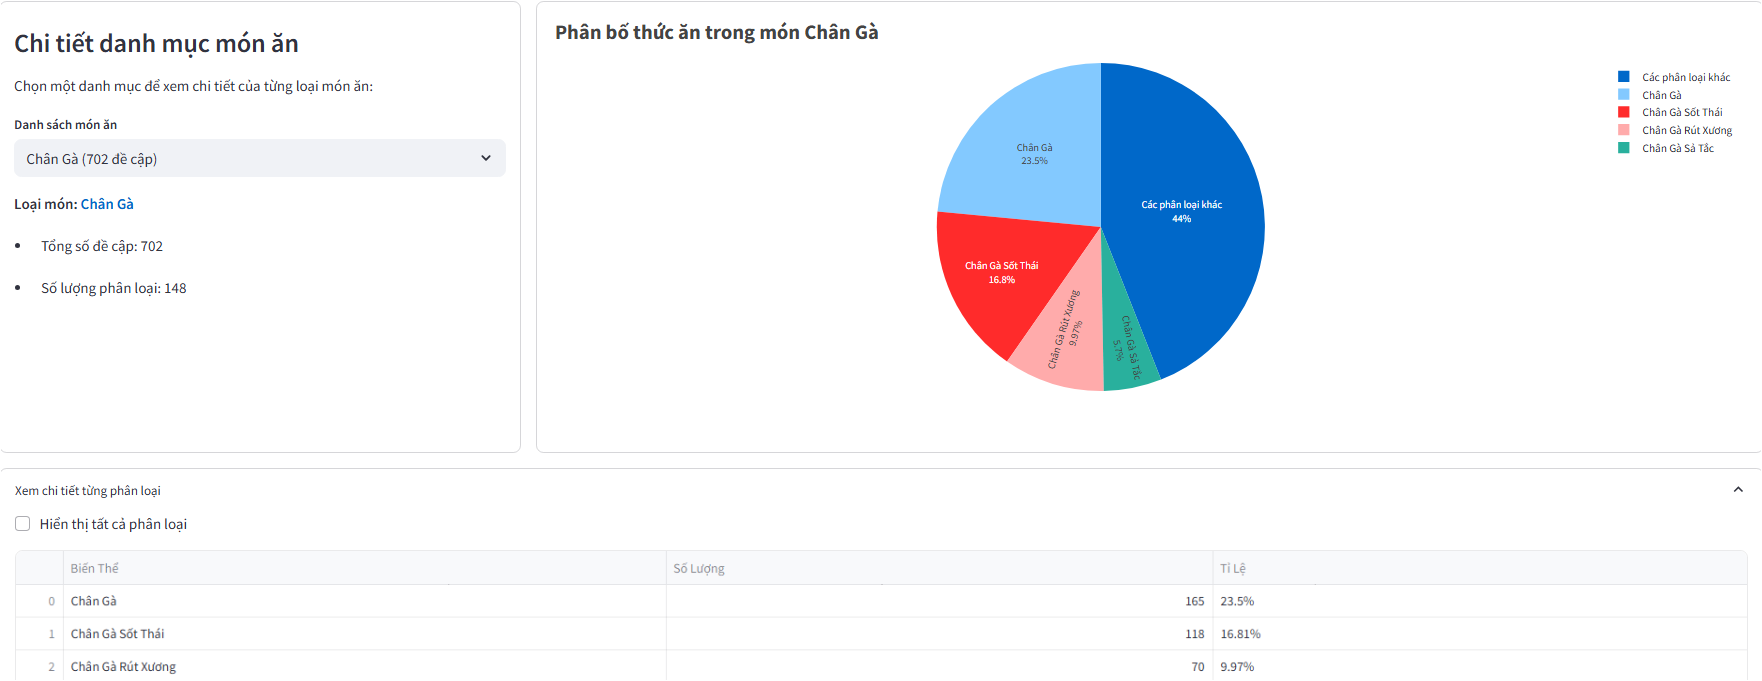
\includegraphics[width=0.99\textwidth]{img/phan_loai.png}}
    \caption{Phân loại các loại \textbf{Chân gà} khác nhau}
    \label{fig:phan_loai}
\end{figure}

Để phân loại món ăn theo danh mục, thay vì sử dụng cách tiếp cận truyền thống với \texttt{dictionary} cố định, nhóm đã phát triển phương pháp phân loại linh hoạt hơn để giải quyết thách thức từ sự đa dạng và biến đổi liên tục của tên món ăn.

Phương pháp này ứng dụng kỹ thuật \texttt{explode} - một hàm cho phép tách các phần tử trong mảng thành các hàng riêng biệt trong DataFrame. Cụ thể:
\begin{enumerate}
    \item Đầu tiên, tên các món ăn được tách thành các từ đơn.
    
    \item Phương thức \texttt{explode} giúp biến đổi mỗi từ trong tên món ăn thành một hàng dữ liệu riêng.
    
    \item Hệ thống sau đó tìm kiếm các cụm từ xuất hiện từ 2 lần trở lên trong tập dữ liệu.
    
    \item Các cụm từ phổ biến này được sử dụng làm cơ sở để tự động tạo và nhóm các danh mục món ăn.
\end{enumerate}

Cách tiếp cận này mang tính thích ứng cao, tự động phát hiện các mẫu hình trong tên món ăn và tạo ra hệ thống phân loại có khả năng mở rộng để đáp ứng với các món ăn mới, độc lạ mà không cần cập nhật thủ công các quy tắc phân loại, đảm bảo hiệu quả trong việc xử lý dữ liệu ẩm thực đa dạng và liên tục thay đổi theo thời gian.

\subsubsection{Phân tích món ăn Nổi bật qua từng tuần}
\begin{figure}[H]
    \centering
    \frame{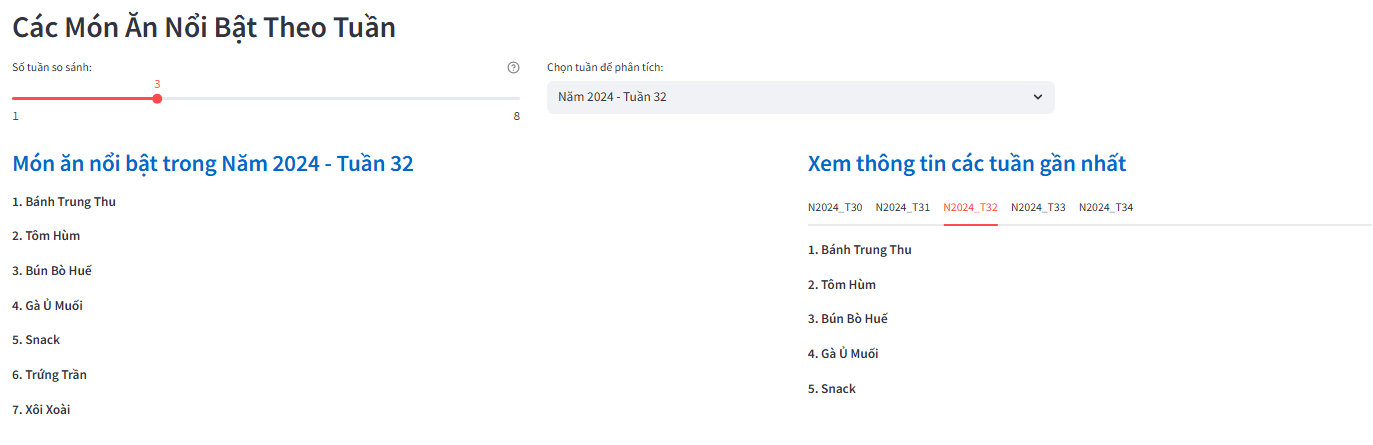
\includegraphics[width=0.99\textwidth]{img/mon_an_noi_bat.png}}
    \caption{Món ăn nổi bật theo từng Tuần}
    \label{fig:mon_an_noi_bat}
\end{figure}

Do các món ăn trong tập dữ liệu đã qua quá trình chọn lọc, đa phần đều có tỷ lệ tương tác cao và xuất hiện trong các video phổ biến, nên mục tiêu của thuật toán là phát hiện những món ăn \textbf{mới} và \textbf{đang thịnh hành} qua từng tuần cụ thể. Dựa trên nền tảng đó, nhóm đã thiết kế thuật toán phân tích dữ liệu ẩm thực theo thời gian nhằm xác định các món ăn đặc trưng cho từng tuần dựa trên phương pháp thống kê thích ứng. 

Phương pháp này cho phép nhận diện các xu hướng ẩm thực nổi bật qua từng giai đoạn thời gian dựa trên các thông số: \textbf{tần suất xuất hiện trong tuần hiện tại}, \textbf{tỷ lệ xuất hiện so với các tuần trước đó}, và \textbf{tổng lượng đề cập}.

\paragraph{Quy trình thực hiện:}
Thuật toán được triển khai theo quy trình sau:
\begin{enumerate}
    \item \textbf{Loại bỏ món ăn phổ biến kéo dài:} Xác định và loại trừ các món ăn xuất hiện trong hơn 60\% tổng số tuần trong tập dữ liệu (70 tuần). Các món này được xem là phổ biến nhưng không phải xu hướng mới.
    
    \item \textbf{Phân tích đặc trưng theo từng tuần:} Xử lý theo hai trường hợp chính:
    \begin{itemize}
        \item \textbf{Trường hợp tuần đầu tiên:} Khi không có dữ liệu để so sánh, thuật toán lấy 10 món ăn được đề cập nhiều nhất làm món đặc trưng.
        
        \item \textbf{Trường hợp các tuần tiếp theo:} So sánh dữ liệu với $n$ tuần trước đó (người dùng có thể điều chỉnh $n$ từ 1 đến 8 tuần). Sau đó áp dụng ba ngưỡng thích ứng:
        \begin{itemize}
            \item \textbf{Ngưỡng 1:} $\geq 3$ lần xuất hiện, chiếm $\geq 60\%$ tổng số lần xuất hiện.
            \item \textbf{Ngưỡng 2:} $\geq 2$ lần xuất hiện, chiếm $\geq 50\%$ tổng số lần xuất hiện.
            \item \textbf{Ngưỡng 3:} $\geq 1$ lần xuất hiện, chiếm $\geq 40\%$ tổng số lần xuất hiện.
        \end{itemize}
    \end{itemize}
    
    \item Nếu thu được đủ 5 món ăn đặc trưng tại một ngưỡng, thuật toán dừng xử lý. Nếu không, tiếp tục hạ ngưỡng để đảm bảo mỗi tuần đều có các món ăn đặc trưng được xác định.
    
    \item Nếu không có món ăn nào đạt bất kỳ ngưỡng nào, thuật toán chọn 5 món có tần suất xuất hiện cao nhất trong tuần hiện tại.
\end{enumerate}

\paragraph{Ưu điểm của phương pháp:}
\begin{itemize}
    \item Tự động điều chỉnh các ngưỡng phân tích phù hợp với đặc điểm phân phối dữ liệu, thích ứng với sự thay đổi của xu hướng ẩm thực theo thời gian.
    
    \item Tách biệt các món ăn phổ biến thường xuyên xuất hiện, tập trung vào các món mới nổi.
    
    \item Vẫn xác định được món đặc trưng ngay cả khi dữ liệu thiếu hoặc không đồng đều, đảm bảo tính liên tục trong phân tích.
\end{itemize}
